\tikzposterlatexaffectionproofoff
\usetheme{Default}

\definecolor{unired}{HTML}{a51e37}
\definecolor{mypink1}{rgb}{0.858, 0.188, 0.478}
\definecolor{mblack}{HTML}{0d0d0d}
\definecolor{titlecolor}{RGB}{74, 114, 159}
\definecolor{titledarkcolor}{RGB}{51,102,153}
\definecolor{Grey}{HTML}{e1e1e1}
\definecolor{DarkerGrey}{RGB}{215,217,219}
\definecolor{FontColor}{HTML}{0d0d0d}
\definecolor{Red}{RGB}{204,0,0}
\definecolor{L-lig}{RGB}{25,124,192}
\definecolor{point-lig}{RGB}{255,255,255}
\definecolor{G-lig}{RGB}{62,66,68}

\definecolor{Orange}{RGB}{240,163,10} 
\definecolor{LightRed}{RGB}{214,98,93}
\definecolor{LightBlue}{RGB}{160,200,217}
\definecolor{LightGreen}{RGB}{130,161,119}
\definecolor{Violet}{RGB}{190,144,252}

\colorlet{blocktitlefgcolor}{mblack}
\colorlet{backgroundcolor}{Grey}
\colorlet{blocktitlebgcolor}{Grey}
\colorlet{blockbodyfgcolor}{FontColor}
\colorlet{innerblocktitlebgcolor}{L-lig}
\colorlet{innerblocktitlefgcolor}{white}
\colorlet{notefrcolor}{white}
\colorlet{notefgcolor}{black}
\colorlet{notebgcolor}{white}


% Title setup
\settitle{ 
\begin{minipage}[b]{0.8\linewidth}
\vspace{2cm}
\hspace{1cm}\color{mblack}{ \Huge{\textbf{\@title}} \par } \vspace*{2em} \hspace{1cm}\color{mblack}{\LARGE \@author \par} \vspace*{2em} \hspace{1cm}{\Large \@institute}\vspace{0.5cm} \end{minipage}

% Add institution logo
\hfill
\begin{minipage}[t]{0.2\linewidth}

    \vspace{-14.3cm}\hspace{-2.8cm}
    
\includegraphics[scale=0.9]{figs/logo_all.pdf}
    
    \vspace{1.2cm}\hspace{8cm}
    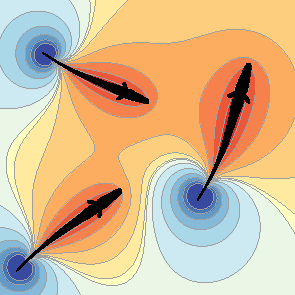
\includegraphics[scale=1.4]{figs/efishlogo.pdf}    

\end{minipage}}

% define title style with background box (currently white)
\definetitlestyle{sampletitle}{
width=841mm, roundedcorners=0, linewidth=0pt, innersep=15pt,
titletotopverticalspace=0mm, titletoblockverticalspace=5pt
}{\begin{scope}[line width=\titlelinewidth, rounded corners=\titleroundedcorners]\draw[fill=point-lig, color=point-lig]
(\titleposleft,\titleposbottom) rectangle (\titleposright,\titlepostop);
\end{scope}}

 % Title, Author, Institute
\title{\parbox{1500pt}{Complex frequency modulations in freely interacting electric fish, \textit{Apteronotus leptorynchus}, recorded in their natural habitat}}
\author{Patrick Weygoldt, Till Raab, Jan Benda}
\institute{Neuroethology Lab, Department of Neurobiology, University of Tuebingen}
\usetitlestyle[]{sampletitle}

% define coustom block style
\defineblockstyle{MyBlock}{% define a custom style for a block
    titlewidthscale=1, bodywidthscale=1, titlecenter,
    titleoffsetx=0pt, titleoffsety=-30pt, bodyoffsetx=0pt, bodyoffsety=-40pt,
    bodyverticalshift=0mm, roundedcorners=25, linewidth=1pt,
    titleinnersep=20pt, bodyinnersep=38pt
}{
    \draw[rounded corners=\blockroundedcorners, inner sep=\blockbodyinnersep,
          line width=\blocklinewidth, color=white,
          top color=titlebgcolor!90, bottom color=titlebgcolor!20!white,
          ]
      (blockbody.south west) rectangle (blockbody.north east); %
    \ifBlockHasTitle%
        \draw[rounded corners=\blockroundedcorners, inner sep=\blocktitleinnersep,
          top color=Grey, bottom color=Grey,
          line width=2, color=Grey, %fill=blocktitlebgcolor
          ]
      (blocktitle.south west) rectangle (blocktitle.north east); %
    \fi%
}
\newcommand\myblock[3][MyBlock]{\useblockstyle{#1}\block{#2}{#3}\useblockstyle{Default}}